\section{Formattatore SAM}

\subsection{Cos'è e come funziona}
Come già detto, gli allineamenti ottenuti dallo Splice-Aware aligner sono in un formato non standard chiamato MEM (nota: l'acronimo MEM si riferisce sia al formato dell'output che all'estensione del file ottenuto). L'obiettivo di questa seconda parte è quello di convertire i due file MEM in un singolo file SAM (Sequence Alignment Map), il formato standard per memorizzare gli allineamenti.

Non si tratta solo di una semplice conversione, in quanto è necessario indurre diverse informazioni aggiuntive per avere un file SAM standard, quali: la posizione di inizio dell'allineamento sulla genomica, la stringa CIGAR, i flag relativi all'allineamento, ecc. Per supportare le read paired-end è stato necessario modificare gran parte di queste funzionalità.

In questa sezione saranno descritte le principali modifiche apportate al Formattatore SAM, oltre ad alcune funzionalità aggiuntive utili per la rilevazione di eventi di Alternative Splicing.

\newpage

\subsection{Modifiche alla computazione del campo FLAG}
Il campo FLAG è il secondo del formato SAM e consiste di un valore numerico (ottenuto convertendo in decimale una serie di flag binari) che rappresenta le caratteristiche dell'allineamento preso in esame. La seguente immagine mostra il significato di ciascun bit del flag:

\begin{figure}[h]
	\centering
	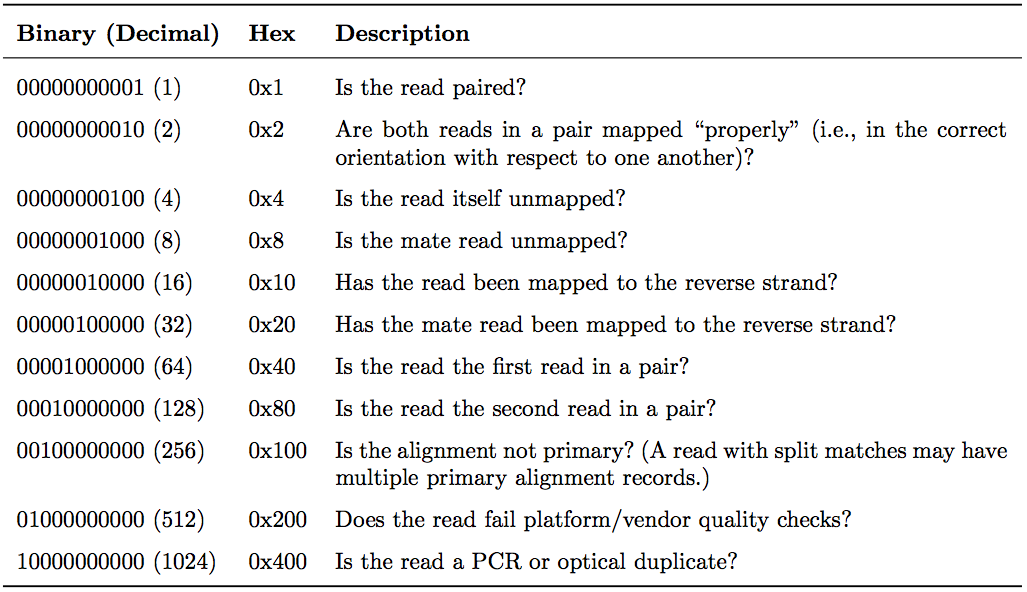
\includegraphics[width=\linewidth]{images/samflag.png}
  \caption{Il significato di ciascun bit del campo FLAG }
  \label{fig:SAM Flags}
\end{figure}

Nei casi single-end solo due flag vengono utilizzati: quello relativo allo strand (0x16) e quello relativo al tipo di allineamento (0x100); visto che le read non sono paired, il flag 0x1 sarà sempre false, quindi tutti i flag risultanti saranno pari.

Nei casi paired-end tutti i flag vengono utilizzati. E' inoltre necessario trattare gli allineamenti a coppie, in quanto il campo FLAG esprime informazioni anche sul mate e non solo sull'allineamento preso in esame. 

Supponiamo ad esempio di avere due read, la prima che mappa sullo strand positivo e la seconda che non mappa (ed è quindi \textit{unmapped}). Sarà innanzitutto necessario mettere a true il flag relativo alle read paired-end (0x1) per entrambe le read. Considerando la prima, sarà messo a true il flag relativo al mate unmapped (0x8) e il flag relativo al first-in-pair (0x4). Considerando la seconda, sarà messo a true il flag relativo alla read unmapped (0x4) e quello relativo al second-in-pair(0x80). I flag in decimale saranno quindi 73 e 133.

Si noti che per il momento non viene tenuto conto dei flag 0x200 e 0x400, ma questo non è di alcuna rilevanza al fine di identificare eventi di Alternative Splicing.

\newpage

\subsection{Calcolo dell' IDMP medio}
Considerando una coppia di read, si definisce IDMP (Inner Distance between Mate Pairs) la distanza sul genoma di riferimento in termini di BP (Base Pair) tra l'ultima base della prima read e la prima della seconda. Questa informazione viene generalmente fornita dall'ente che ha effettuato il sequenziamento, e può essere confrontata con l'IDMP medio rilevato durante l'allineamento per rilevare nuovi eventi di Alternative Splicing.

Prima di poter calcolare l'IDMP è necessario introdurre il concetto di BitVector, ovvero una sequenza di bit che rappresenta la posizione degli esoni nella genomica. Un BitVector è dotato di due operazioni:

\begin{itemize}
	\item Rank: data una posizione, ritorna l'esone di provenienza
	\item Select: dato un esone, ritorna la posizione di partenza 
\end{itemize}



\newpage

\subsection{Calcolo del TIDMP}

\newpage

\subsection{Calcolo delle statistiche dell'allineamento}

\newpage